\documentclass[12pt,twoside]{article}
%%%%%%%%%%%%%%%%%%%%%%%%%%%%%%%%%%%%%%%%%%%%%%%%%%%%%%%%%%%%%
% Meta informations:
\newcommand{\trauthor}{Soubarna Banik}
\newcommand{\trtype}{Project Report} %{Seminararbeit} %{Proseminararbeit}
\newcommand{\trcourse}{Independent Study}
\newcommand{\trtitle}{Superpixel-based Road Detection using Hyperspectral Images}
\newcommand{\trmatrikelnummer}{6640587}
\newcommand{\tremail}{4banik@informatik.uni-hamburg.de}
\newcommand{\trarbeitsbereich}{Cognitive Systems Laboratory, KOGS}
\newcommand{\trdate}{08.05.2017}

%%%%%%%%%%%%%%%%%%%%%%%%%%%%%%%%%%%%%%%%%%%%%%%%%%%%%%%%%%%%%
% Languages:

% Falls die Ausarbeitung in Deutsch erfolgt:
% \usepackage[german]{babel}
% \usepackage[T1]{fontenc}
% \usepackage[latin1]{inputenc}
% \usepackage[latin9]{inputenc}	 				
% \selectlanguage{german}

% If the thesis is written in English:
\usepackage[english]{babel} 						
\selectlanguage{english}

%%%%%%%%%%%%%%%%%%%%%%%%%%%%%%%%%%%%%%%%%%%%%%%%%%%%%%%%%%%%%
% Bind packages:
\usepackage{acronym}                    % Acronyms
\usepackage{algorithmic}								% Algorithms and Pseudocode					
\usepackage{algorithm2e}
\usepackage{amsfonts}                   % AMS Math Packet (Fonts)
\usepackage{amsmath}                    % AMS Math Packet
\usepackage{amssymb}                    % Additional mathematical symbols
\usepackage{amsthm}
\usepackage{booktabs}                   % Nicer tables
\usepackage[font=small,labelfont=bf]{caption} % Numbered captions for figures
\usepackage{color}                      % Enables defining of colors via \definecolor
\definecolor{uhhRed}{RGB}{254,0,0}		  % Official Uni Hamburg Red
\definecolor{uhhGrey}{RGB}{122,122,120} % Official Uni Hamburg Grey
\usepackage{fancybox}                   % Gleichungen einrahmen
\usepackage{fancyhdr}										% Packet for nicer headers
%\usepackage{fancyheadings}             % Nicer numbering of headlines

%\usepackage[outer=3.35cm]{geometry} 	  % Type area (size, margins...) !!!Release version
%\usepackage[outer=2.5cm]{geometry} 		% Type area (size, margins...) !!!Print version
%\usepackage{geometry} 									% Type area (size, margins...) !!!Proofread version
\usepackage[outer=3.15cm]{geometry} 	  % Type area (size, margins...) !!!Draft version
\geometry{a4paper,body={5.8in,9in}}

\usepackage{graphicx}                   % Inclusion of graphics
\usepackage{wrapfig}

%\usepackage{latexsym}                  % Special symbols
\usepackage{longtable}									% Allow tables over several parges
\usepackage{listings}                   % Nicer source code listings
\usepackage{multicol}										% Content of a table over several columns
\usepackage{multirow}										% Content of a table over several rows
\usepackage{rotating}										% Alows to rotate text and objects
\usepackage[hang]{subfigure}            % Allows to use multiple (partial) figures in a fig
%\usepackage[font=footnotesize,labelfont=rm]{subfig}	% Pictures in a floating environment
\usepackage{tabularx}										% Tables with fixed width but variable rows
\usepackage{url,xspace,boxedminipage}   % Accurate display of URLs
%%%%%%%%%%%%%%%%%%%%%%%%%%%%%%%%%%%%%%%%%%%%%%%%%%%%%%%%%%%%%
% Configurationen:

\hyphenation{whe-ther} 									% Manually use: "\-" in a word: Staats\-ver\-trag

%\lstloadlanguages{C}                   % Set the default language for listings
\DeclareGraphicsExtensions{.pdf,.svg,.jpg,.png,.eps} % first try pdf, then eps, png and jpg
\graphicspath{{./src/}} 								% Path to a folder where all pictures are located
\pagestyle{fancy} 											% Use nicer header and footer

% Redefine the environments for floating objects:
\setcounter{topnumber}{3}
\setcounter{bottomnumber}{2}
\setcounter{totalnumber}{4}
\renewcommand{\topfraction}{0.9} 			  %Standard: 0.7
\renewcommand{\bottomfraction}{0.5}		  %Standard: 0.3
\renewcommand{\textfraction}{0.1}		  	%Standard: 0.2
\renewcommand{\floatpagefraction}{0.8} 	%Standard: 0.5

% Tables with a nicer padding:
\renewcommand{\arraystretch}{1.2}

%%%%%%%%%%%%%%%%%%%%%%%%%%%%
% Additional 'theorem' and 'definition' blocks:
\theoremstyle{plain}
\newtheorem{theorem}{Theorem}[section]
%\newtheorem{theorem}{Satz}[section]		% Wenn in Deutsch geschrieben wird.
\newtheorem{axiom}{Axiom}[section] 	
%\newtheorem{axiom}{Fakt}[chapter]			% Wenn in Deutsch geschrieben wird.
%Usage:%\begin{axiom}[optional description]%Main part%\end{fakt}

\theoremstyle{definition}
\newtheorem{definition}{Definition}[section]

%Additional types of axioms:
\newtheorem{lemma}[axiom]{Lemma}
\newtheorem{observation}[axiom]{Observation}

%Additional types of definitions:
\theoremstyle{remark}
%\newtheorem{remark}[definition]{Bemerkung} % Wenn in Deutsch geschrieben wird.
\newtheorem{remark}[definition]{Remark} 

%%%%%%%%%%%%%%%%%%%%%%%%%%%%
% Provides TODOs within the margin:
\newcommand{\TODO}[1]{\marginpar{\emph{\small{{\bf TODO: } #1}}}}
\newcommand{\forceindent}{\leavevmode{\parindent=2em\indent}}
%%%%%%%%%%%%%%%%%%%%%%%%%%%%
% Abbreviations and mathematical symbols
\newcommand{\modd}{\text{ mod }}
\newcommand{\RS}{\mathbb{R}}
\newcommand{\NS}{\mathbb{N}}
\newcommand{\ZS}{\mathbb{Z}}
\newcommand{\dnormal}{\mathit{N}}
\newcommand{\duniform}{\mathit{U}}

\newcommand{\erdos}{Erd\H{o}s}
\newcommand{\renyi}{-R\'{e}nyi}
%%%%%%%%%%%%%%%%%%%%%%%%%%%%%%%%%%%%%%%%%%%%%%%%%%%%%%%%%%%%%
% Document:
\begin{document}
\renewcommand{\headheight}{14.5pt}

\fancyhead{}
\fancyhead[LE]{ \slshape \trauthor}
\fancyhead[LO]{}
\fancyhead[RE]{}
\fancyhead[RO]{ \slshape \trtitle}

%%%%%%%%%%%%%%%%%%%%%%%%%%%%
% Cover Header:
\begin{titlepage}
	\begin{flushleft}
		Universit\"at Hamburg\\
		Department Informatik\\
		\trarbeitsbereich\\
	\end{flushleft}
	\vspace{3.5cm}
	\begin{center}
		\huge \trtitle\\
	\end{center}
	\vspace{3.5cm}
	\begin{center}
		\normalsize\trtype\\
		[0.2cm]
		\Large\trcourse\\
		[1.5cm]
		\Large \trauthor\\
		[0.2cm]
		\normalsize Matr.Nr. \trmatrikelnummer\\
		[0.2cm]
		\normalsize\tremail\\
		[1.5cm]
		\Large \trdate
	\end{center}
	\vfill
\end{titlepage}

	%backsite of cover sheet is empty!
\thispagestyle{empty}
\hspace{1cm}
\newpage

%%%%%%%%%%%%%%%%%%%%%%%%%%%%
% Abstract:

% Abstract gives a brief summary of the main points of a paper:
\section*{Abstract}
In this paper, a superpixel based unsupervised road detection system, using remotely sensed hyperspectral images is proposed. The model is computationally efficient as it operates on superpixels rather than individual pixels. The use of hyperspectral images helps to identify roads accurately by utilizing the knowledge of the reflectance spectra of materials used in construction of roads. The model aims to eliminate the dependency on human intervention, and follows an unsupervised approach. 
% Lists:
\setcounter{tocdepth}{2} 					% depth of the table of contents (for Seminars 2 is recommented)
\tableofcontents
\pagenumbering{arabic}
\clearpage

%%%%%%%%%%%%%%%%%%%%%%%%%%%%
% Content:

% the actual content, usually separated over a number of sections
% each section is assigned a label, in order to be able to put a
% crossreference to it

\section{Introduction}
\label{sec:introduction}
Advances in hyperspectral imaging technologies have opened up an entirely new way of looking at our planet, and have added considerably to our knowledge about it. Hyperspectral spectrometers capture high resolution images consisting usually of more than a hundred bands/channels. Remotely sensed RGB or multispectral data often do not provide sufficient information for differentiating similar looking materials. Also the task is more complex as the images are captured from such high altitudes. The unique continuous reflectance spectra of different materials has made it possible to identify target materials from remotely sensed hyperspectral images. Its benefit can be reaped across a variety of applications, such as vegetation identification, agricultural monitoring, atmospheric and ocean characteristics study, mineral exploration and environmental monitoring. Another key application of remote sensing is urban monitoring. As per the World Health Organisation (WHO) the urban population in 2014 accounted for 54\% of  the total global population \footnote{\url{http://www.who.int/gho/urban_health/situation_trends/urban_population_growth_text/en/}}. This rapid growth needs to be monitored to ensure urban planning, future development and sustainable growth. 
Road network identification is an important aspect of urban monitoring as it can be considered as a measure of urbanization. It also provides significant information for planning transportation. Most of the current road mapping algorithms require manual intervention, which is a tedious and time-consuming processes.\\
\forceindent With hundreds of bands, hyperspectral images suffer from the problem of high data dimensionality. Though state of the art machine learning algorithms can overcome this problem, it is not always possible to acquire enough hyperspectral data samples as acquiring these images is a costly process. Also, the measurements of the individual pixels are often prone to noise and intra-class variability of spectra \cite{thompson2010superpixel}. Superpixel segmentation acts as a solution to both problems of high data dimensionality and noise. The term "superpixel" was introduced by Ren and Malik in \cite{ren2003learning} to indicate a group of pixels that are local and coherent in features. By representing a set of pixels with a single superpixel, the data redundancy in images reduces considerably. It is also beneficial to run optimization algorithms on superpixels rather than at pixel level, which is computationally expensive, and at times infeasible due to large number of pixels in high resolution images. Ren and Malik also argue in \cite{ren2003learning} that pixels are mere results of image discretization and they are not natural entities. Superpixels produce an image representation that is closer to human perception. In the context of hyperspectral data, a superpixel's mean spectra represents the component pixels' individual reflectance spectra. Computation of the mean spectra acts as a smoothing operation, thereby reducing the pixel level noise. A large superpixel will reduce the noise effect best, however, as pointed out by Gilmore et al.\cite{gilmore2011superpixel}, it may also overshadow small features that may have cropped up due to presence of distinct materials. Classification of hyperspectral data at the superpixel level, hence, reduces the computational complexity, as well as reduces the effect of noise.\\
\forceindent In this paper, a fully automatic superpixel-based road detection algorithm is proposed. The paper is organized as follows - section \ref{sec:relatedwork} gives a description of the existing road extraction models. Hyperspectral image and its characteristics are described in section \ref{sec:HypTheo}. Section \ref{sec:dataset} introduces the dataset used. Section \ref{sec:model} depicts the proposed superpixel based road extraction method and section \ref{sec:experiment} evaluates the experimental results. Section \ref{sec:concl} contains concluding remarks.

\section{Related Work}
\label{sec:relatedwork}
Over the last three decades, a lot of work has been done on techniques for road detection, road network extraction and road centerline determination. These techniques were broadly categorised by Poullis et al. in \cite{Poullis2010} into three categories - pixel based, region based and knowledge based techniques. The pixel-based methods operate directly on the pixels. Most of the initial work on road detection was pixel based. Examples of the recent pixel based techniques are road network detection from multispectral imagery by Zhang et al. \cite{Zhang2006} and a vision-based system for automatic road detection by Poullis et al. \cite{Poullis2010}. The region-based methods segment the images into regions, and operate on the regions in stead of the individual pixels, thereby reducing the computation cost. Some of the region based approaches are a higher order CRF(conditional random field) model based on superpixels by Wegner et al. \cite{Wegner2013}, a graph based road tracking system by Seppke et al. \cite{Seppke2016} and a road centerline extraction model using multiscale segmentation and tensor voting by Cheng et al. \cite{Cheng}. The knowledge-based methods take some higher level information into consideration - such as the geometric and radiometric properties of road, or some contextual information.\\
\forceindent Road detection systems can also be grouped into semi-automatic and fully automatic approaches. Semi-automatic approaches rely on initial seed points for tracking or require some intervention by a human operator. For example, the previously mentioned method in \cite{Seppke2016} relies on initial seed points. On the other hand the fully automatic approaches need no such human intervention. In addition to this, there are supervised and unsupervised road classification methods. The supervised approaches need labelled data, and as ground truth determination is a very tedious process, its availability is scarce. Unsupervised fully automatic approaches overcome these hurdles, however, novel validation techniques are required in order to avoid dependency on labelled ground truth data.\\
\forceindent Many of the road detection approaches utilize different geometric properties of roads to improve the models' performance. Two such common properties are the linearity and large area of road segments. For example, Miao et al. use \textit{linear feature index} (LFI), a ratio of the length and width of the minimum bounding box of a segment in \cite{Miao2013}. Cheng et al. use three different shape features in \cite{Cheng} : \textit{shape index} (SI) - a ratio of perimeter and area of a segment, \textit{aspect ratio} (AR) - ratio of the length and width of the bounding box of segments, and \textit{elliptical LFI} - where the ratio is computed for the bounding ellipse in stead of the bounding box. Though Cheng et al. have argued against the normal LFI, the aspect ratio feature used by them is similar to the LFI feature. Few other properties that have been utilised in research are the ratio of segment area and bounding box area, circularity and convexity of segments. Looking at the various pros and cons of the above mentioned approaches, a region based unsupervised approach for road detection is proposed in this paper. The proposed model utilizes the hyperspectral and geometric properties of roads for detection.

\section{Hyperspectral Image}
\label{sec:HypTheo}
Before the advent of hyperspectral imaging, multispectral imaging was used to analyze target materials in electromagnetic (EM) wavebands, in addition to the widely used visible (red, green and blue) wavebands. A hyperspectral or multispectral spectrometer measures the reflectance of target materials - the percentage of incident radiation that is reflected by the material. A reflectance spectrum shows the reflectance of a material measured across a range of wavelengths \cite{shippert2003introduction}. The satellite sensors, Landsat Thematic Mapper and SPOT XS,  produce multispectral images. Unlike hyperspectral images, multispectral images constitute of fewer  and relatively broad bands. For example, the SPOT XS multispectral images have bandwidth in the range of $10 \mu m$ and consists of 4 such bands. On the other hand, hyperspectral spectrometers acquire images in much narrower bands ($10-20nm$). The narrower and contiguous bands of hyperspectral images helps in creating continuous spectrum which uniquely identifies each material. Each material responds differently to the incident radiations - in some wavelengths, its reflectance is high, whereas some other material absorbs highly in the same wavelengths.\\
\forceindent \textit{Hyperspectral Cube:} A hyperspectral image is usually represented as a cube, containing two spatial dimensions and one spectral dimension. 
\begin{wrapfigure}{l}{0.55\textwidth}
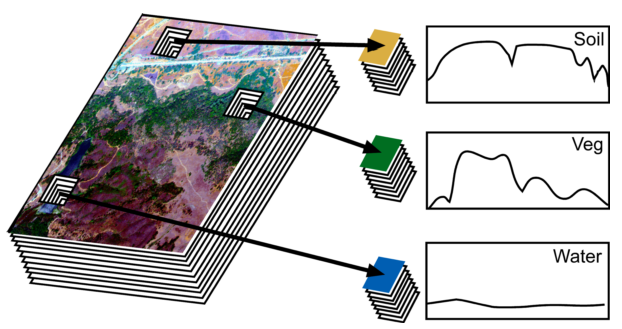
\includegraphics[width=0.55\textwidth]{src/Hyperspectral_cube.png}
\caption{Hyperspectral cube and a plot of reflectance spectrum of three pixels \cite{shippert2003introduction}}
\label{fig:hyp_cube}
\end{wrapfigure}
The spectral dimension consists of many narrow, adjacent wavelength bands. Figure \ref{fig:hyp_cube} shows a sample hyperspectral cube and the reflectance spectra of three sample pixels against the EM wavelengths. It can be seen, the spectral signature is different for the three different materials - soil, vegetation and water and thus, these materials can be identified by their reflectance spectra.
\begin{figure}[hbtp]
\centering
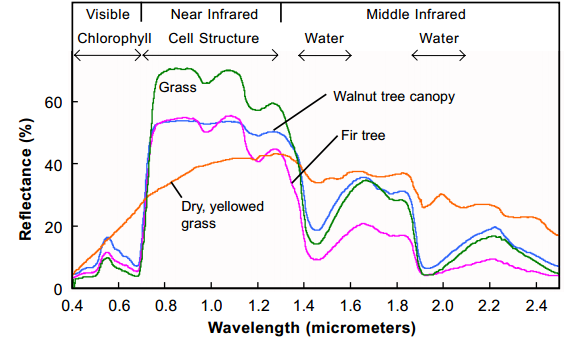
\includegraphics[width=0.75\textwidth]{src/plant_spectra.png}
\caption{Reflectance spectra of different types of plants. \cite{smith2012} }
\label{fig:plant_spec}
\end{figure}
Even materials belonging to the same class differ in their spectra. For example, different plant species have different spectral signatures due to varied leaf structure, chlorophyll and water content etc. As seen in Figure \ref{fig:plant_spec}, the spectral signatures for trees, grass, even dry yellowed grass differ, though these belong to the same class, vegetation. Different components of plants contribute to different portions of the spectra.\\
\forceindent \textit{Spectral Libraries and Classification:} There are several spectral libraries available that consist of collections of reflectance spectra of natural as well as composite materials of known compositions. Besides, different datasets are also accompanied by their own spectral libraries, containing the spectra for the materials in the corresponding field site. Some of the well-known public spectral libraries are ASTER spectral library by NASA \cite{baldridge2009aster} and USGS spectral library by the United States Geological Survey Spectroscopy Lab \cite{clark1993us}. Spectral libraries are used to classify different materials in hyperspectral images. The reflectance spectra of hyperspectral pixels are compared with the spectral library to identify the nearest matching constituent material.\\
\forceindent \textit{Spectral Unmixing:} Often, due to the limited spatial resolution of a hyperspectral image, several materials contribute towards the spectrum of a pixel and it becomes hard to classify the pixel from its reflectance spectrum.
\begin{figure}[hbtp]
\centering
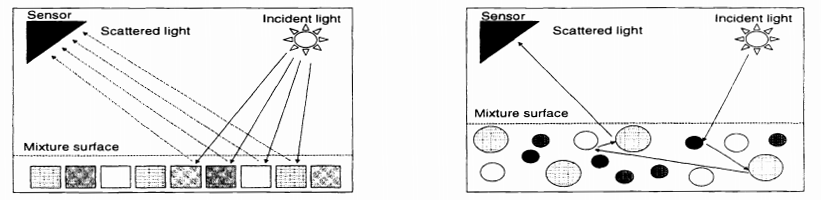
\includegraphics[width=0.95\textwidth]{src/spectral_unmixing.png}
\caption{Spectral unmixing: linear mixing from a checkerboard mixture having a single reflection (left), non-linear mixing from an intimate mixture having multiple reflections (right) \cite{keshava2000algorithm}}
\label{fig:unmix}
\end{figure}
In this scenario, a method called spectral unmixing is applied to quantify the proportion of each contributing material in a pixel. Spectral unmixing algorithms generate an abundance map, which reports the percentage of all the pure surface materials, also called endmembers, for every pixel. An endmember's contribution is also known as abundance fraction. Spectral unmixing algorithms can be both linear and non-linear. The linear algorithms are applied in case of  a checkerboard mixture of materials in a pixel, where the materials lie side by side. In such a mixture, incident rays reflect only once from the surface, yielding a linear relationship between the fractional abundance and the reflected spectra \cite{keshava2000algorithm}. In case of a random mixture of materials, the incident rays are reflected multiple times by the materials, thereby producing a non-linear relationship between the final reflected spectra and the abundance fractions. This is depicted in Figure \ref{fig:unmix}.

\section{Dataset}
\label{sec:dataset}
The dataset used to test the proposed model is the Berlin-Urban-Gradient dataset \cite{okujeni2016berlinurbangradient}, a ready-to-use multi-scale imaging spectrometer dataset prepared by GFZ German Research Center for Geosciences. The dataset contains two hyperspectral scenes, named HyMap01 and HyMap02, at 3.6m and 9m resolution respectively. The two scenes were captured by the German Aerospace Center (DLR) on 20 August 2009 around solar noon under a clear sky condition. These two scenes can be referred to in Figure \ref{fig:data}.
\begin{figure}[hbtp]
\centering
\includegraphics[width=0.85\textwidth]{src/Berlin_Urban_Gradient_2009_Coverage2.png}
\caption{Coverage of HyMap scenes in Berlin-Urban-Gradient dataset \cite{okujeni2016berlinurbangradient}}
\label{fig:data}
\end{figure}
\\ \forceindent A spectral library of 75 relevant materials is also provided with the dataset. The spectral library is structured in a two level hierarchy. The first level groups the library into four categories - namely \textit{impervious, vegetation, soil} and \textit{other}. The second level further categorizes the \textit{impervious} into \textit{roof} and \textit{pavement}, and \textit{vegetation} into \textit{low vegetation} and \textit{tree}. The level 2 category \textit{pavement} is built of four varieties of asphalt and three varieties of concrete. The proposed algorithm is tested on parts of HyMap02, the lower resolution scene. The image provided in the dataset is already preprocessed. The pre-processing steps include system correction, atmospheric correction, parametric geocoding and noisy band removal \cite{okujeni2016berlinurbangradient}. The HyMap02 contains 111 bands over the range of $0.4554\mu m - 2.4465\mu m$.

\section{Road Detection using Hyperspectral Image}
\label{sec:model}
In this section, the proposed superpixel based road detection method is described. The architecture of the model is shown in Figure \ref{fig:arch}. The method can be divided into four main stages - an initial superpixel over-segmentation, followed by a post-processing phase, a classification phase and a final post-processing phase.
\begin{figure}[hbtp]
\centering
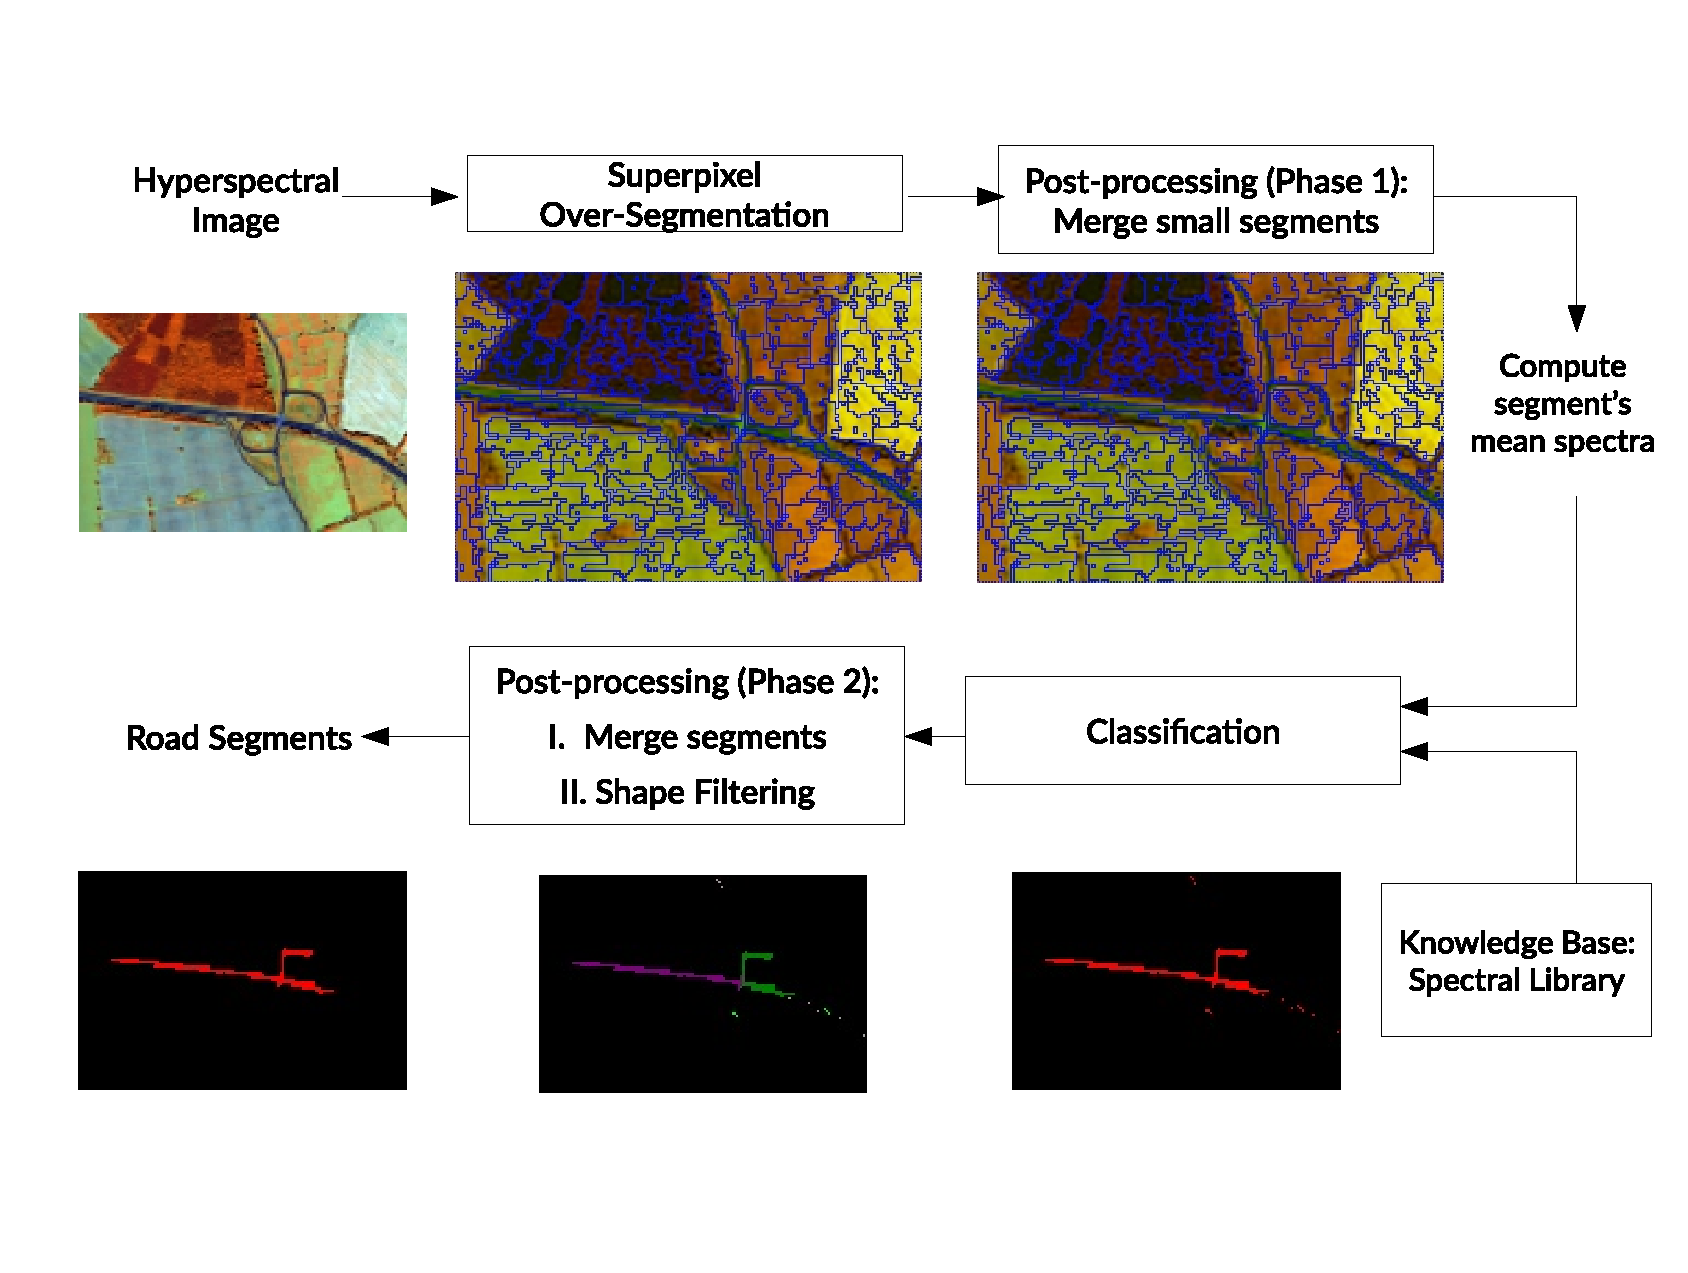
\includegraphics[width=\textwidth]{src/architecture2.eps}
\caption{Architecture of the proposed road detection model using hyperspectral image}
\label{fig:arch}
\end{figure}
The superpixel segmentation phase overly segments the input hyperspectral image. The post-processing phase merges small noisy segments. The classification phase classifies the segments into the six categories from the spectral library, mentioned in section \ref{sec:dataset} - roof, pavement, low vegetation, tree, soil and others. The final post-processing step merges small candidate road segments and filters segments according to the linear shape.

\subsection{Superpixel Over-Segmentation}
For superpixel segmentation, the graph-based segmentation algorithm by Felzenszwalb and Huttenlocher \cite{felzenszwalb2004efficient} was chosen. In this graph-based approach, each pixel is considered as a node, and the weights on edges connecting two nodes signify the distance between them in feature space. Felzenszwalb's algorithm performs a merge operation on the nodes to form the superpixels, with the constraint that each superpixel is a minimum spanning tree of the constituent pixels. For the proposed model, Felzenszwalb's segmentation algorithm has been adapted for hyperspectral images.

\subsubsection{Segmentation algorithm of Felzenszwalb and Huttenlocher}
\label{sec:felz}
In this section, the original algorithm \cite{felzenszwalb2004efficient} is explained. The input image is represented as a graph $G = (V,E)$, with $n$ vertices, $V$ and $m$ edges, $E$. Each node signifies a pixel in the image and an edge connects neighboring pixels. The weights on edge encode the dissimilarity between the connecting pixels. The algorithm returns a set of segmented components, $S = (C_1,C_2,...C_r)$.\\
\\
\begin{algorithm}[H]
\label{alg:felz}
\SetAlgoLined
\KwData{$G = (V,E)$}
\KwResult{$S_m = \{C_1,C_2...C_r\}$ }
Sort edges $E$ according to weight $\pi = (o_1, o_2....o_m)$\;
Set initial segmentation $S_0 = \{C_0,C_1,...C_n\}$, where every component represents a vertex\;
\Repeat{$q = 1,...m$}{
For $q^{th}$ edge in $\pi$, construct $S_q$ from $S_{q-1}$\;
Set $v_i$ and $v_j$, the connecting vertices of the $q^{th}$ edge, belonging to the components $C_{i}^{q-1}$ and $C_{j}^{q-1}$ in $S_{q-1}$\;
\eIf{$(C_{i}^{q-1} \ne C_{j}^{q-1})$ and $(w(v_i,v_j)<MInt(C_i,C_j))$}{
	Merge $C_i$ and $C_j$ to obtain $S_q$
}{
$S_q=S_{q-1}$
}
}
\caption{Segmentation algorithm of Felzenszwalb and Huttenlocher \cite{felzenszwalb2004efficient}}
\end{algorithm}
\vspace{5mm}
Two measures of dissimilarity, namely the \textit{internal difference}, $Int(C)$ of a component and the \textit{minimum internal difference}, $MInt(C_1,C_2)$ between two components are used to detect a boundary between two components. The internal difference of a component $C$ is the maximum weight in the minimum spanning tree of the component, $MST(C, E)$ \cite{felzenszwalb2004efficient}.
\begin{equation}
\label{eq:int_diff}
Int(C) = max_{e \in MST(C,E)} w(e)
\end{equation}
In order to decide if a boundary exists between two components, the algorithm compares the inter-component difference to components' internal differences and if the former is larger than the minimum internal difference, a boundary is decided. The minimum internal difference between two components is defined as\\
\begin{equation}
\label{eq:mint}
MInt(C_1,C_2) = min(Int(C_1)+\tau(C_1), Int(C_2)+\tau(C_2))
\end{equation}
where, $\tau$ is a threshold function $\tau(C) = \dfrac{k}{\lvert C\rvert}$ and $k$ is a constant parameter. The value of $k$ decides the size of the component - with larger $k$, larger components are created.\\
\forceindent In order to implement Felzenszwalb's algorithm on hyperspectral images, initially each pixel's spectrum, $r$ is represented as a node. The weights of the edges connecting two nodes are calculated using two distance metrics - the Euclidean distance ($d_e$) and the spectral angle distance ($d_{SAD}$) between two pixels' spectra respectively. The experiment was repeated for both distance measures in order to compare the performances. The distance metrics are defined as follows:\\
\forceindent \textit{Eucledian distance:}
\begin{equation}
\label{eq:euc}
d_e(v_i,v_j) = \sqrt{\sum_{\lambda} (r_{i\lambda} - r_{j\lambda})^{2}}
\end{equation}
\forceindent \textit{Spectral Angle distance:}
\begin{equation}
\label{eq:sad}
d_{SAD}(v_i,v_j) = \sum_{\lambda} \dfrac{r_{i\lambda}r_{j\lambda}}{|r_{i\lambda}||r_{j\lambda}|}
\end{equation}
where, $v_i,v_j$ are neighboring pixels, $r_i,r_j$ are the spectra of the pixels and $\lambda$ denotes the band of the hyperspectra. 

\subsection{Post-Processing (Phase 1)}
\label{sub sec:PP1}
The segmentation phase overly segments the input image and generates lot of small superpixels. To get rid of small noisy regions, all superpixels less than a minimum component size, $min\_size$ are merged with its neighboring superpixels. In order to detect the narrow road segments, $min\_size$ threshold is set to a low value. Once the segments are merged, the mean reflectance spectra of all superpixels are computed. These mean spectra are considered as the input for the next stage.

\subsection{Classification}
With the help of the spectral library, the mean spectra of the superpixels are classified. For classification, two alternative approaches were followed - \textit{nearest neighbor classification} and \textit{spectral unmixing}.
\subsubsection{Nearest Neighbor Classification} In this approach, the  nearest neighbor of the superpixel is determined from the spectral library, available in the dataset. To compute the nearest neighbor, the spectral angle distances between the mean spectra of a superpixel and each spectra from the spectral library are computed. As explained in section \ref{sec:dataset}, the spectral library is grouped into several categories. Each of the level 2 categories - roof, pavement, low vegetation, tree, soil and other, contains several spectra. The distance computed at the individual spectral level is averaged to level 2 categories. Finally, the superpixel is mapped to the category with the minimum distance.

\subsubsection{Spectral Unmixing} In this approach, a superpixel is classified using a simple linear spectral unmixing algorithm as in \cite{keshava2002spectral}. The algorithm solves a few linear equations to compute the abundance map for all superpixels. As in \cite{keshava2002spectral} a simple linear mixing model (LMM) is formulated as 
\begin{equation}
\label{eq:LMM}
x = Sa + w
\end{equation}
where $x$ is a $L \times 1$ matrix signifying the $L$ band spectra of a superpixel, $S$ is a $L \times M$ matrix, signifying the spectra of $M$ endmembers from the spectral library, $a$ denotes the $M \times 1$ abundance vector and $w$ is the additive noise vector. As stated by Keshava et al. in \cite{keshava2002spectral}, an abundance vector is subject to two constraints - i) the non-negativity constraint requires all endmember abundance fraction to be non-negative and ii) the full additivity constraint requires the sum of abundance fractions for all endmembers to be $1$.
For classifying the superpixel, first, the unconstrained abundance map, $\hat{a}^U$ is created, assuming zero additive noise, $w$ \cite{keshava2002spectral}. Following the least square minimization of the error $ \lvert x - Sa^U \rvert^2$ as in \cite{keshava2002spectral}, an estimate of the unconstrained abundance vector, $\hat{a}^U$ is obtained:
\begin{equation}
\label{eq:un_abundance}
\hat{a}^U = (S^T S)^{-1} S^T x
\end{equation}
The unconstrained solution is refined by the full-additivity constraint to generate the full-additive abundance vector, $\hat{a}^F$. The equation for full-additive abundance vector is reproduced from \cite{keshava2002spectral} in equation \ref{eq:fa_abundance}.
\begin{equation}
\label{eq:fa_abundance}
\hat{a}^F = \hat{a}^U - (S^T S)^{-1} Z^T [Z(S^T S)^{-1} Z^T]^{-1}(Z \hat{a}^U - b)
\end{equation}
where, $Z$ is an identity matrix of dimension $1 \times M$ and $b = 1$. Further details can be found in the original paper \cite{keshava2002spectral}. The superpixel is mapped to the endmember having the maximum abundance fraction in the abundance vector. Finally, the superpixels that are mapped to the endmembers asphalt and concrete from the Berlin-Urban gradient dataset, are classified as candidate road segments.

\subsection{Post-processing (Phase 2)}
Once the candidate road segments are identified, some post-processing steps are followed to refine the results. In this step, the segments with linear shape are filtered out of the candidate road segments. For shape filtering a basic shape feature indicator is used. For each candidate segment, the ratio of its perimeter and  area is calculated. The linear segments have higher shape feature value than the non-linear. However, due to the low $min\_size$ threshold in the first post-processing phase, the segments generated are small in size, resulting in low shape feature value. In order to avoid this, the neighboring segments are first merged after comparing with a higher threshold value $min\_size2$. Finally, all candidate segments having a shape feature value higher than a threshold are classified as road segments. 

\section{Experimental Result}
\label{sec:experiment}
The proposed method is tested on a sub-region of the HyMap02 scene (row 2000-2400, column 40-630) (Figure \ref{fig:gt}), referred to as scene$1$ henceforth. The scene corresponds to a rural area with few prominent highroads and some city roads. Another sub-region of the HyMap02 scene (row 1500-2000, column 50-630), a relatively more urban area than scene$1$, is chosen as the second test scene. This scene will be referred to as scene$2$.
\begin{figure}[htbp]
\centering     %%% not \center
\subfigure[Input scene, a sub-region from HyMap02 scene (bands R=0.7$\mu m$, G=1.2 $\mu m$, B=0.6$\mu m$)]{\label{fig:seg_in}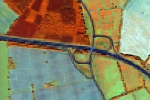
\includegraphics[scale=0.9]{src/seg_input_file1.jpg}}
\subfigure[Output for Euclidean distance metric, $k=100$ and $min\_size=10$]{\label{fig:seg_op_EU}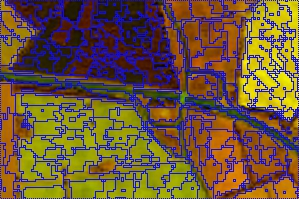
\includegraphics[scale=0.45]{src/segmented_EU_k_100_m_10}}
\subfigure[ Output for SAD distance metric, $k=100$ and $min\_size=10$]{\label{fig:seg_op_SAD}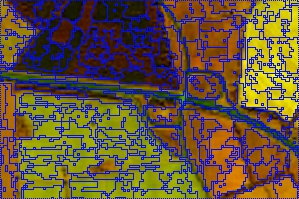
\includegraphics[scale=0.45]{src/segmented_SAD_k_100_m_10.jpg}}
\caption{Segmentation output produced by the modified Felzenszwalb and Huttenlocher algorithm}
\label{fig:seg}
\end{figure}
The model is run for different values of the parameters $k$ and $min\_size$. $k$ is varied from $40$ to $140$ in steps of $10$ and $min\_size$ is varied from $5$ to $20$ in steps of $5$. The parameters $min\_size2$ and the shape feature threshold are empirically decided to $30$ and $0.6$ respectively. The superpixel segmentation output for a sub-section of scene$1$ for both distance metrics, EU and SAD can be found in Figure \ref{fig:seg}.\\
\begin{figure}[htbp]
\label{fig:classify_nn_op}
\centering     %%% not \center
\subfigure[Scene$1$, a rural sub-section from HyMap02 scene in infrared (bands R=1.0014$\mu m$, G=1.0166 $\mu m$, B=1.0318$\mu m$), with ground truth highroads marked in blue]{\label{fig:gt}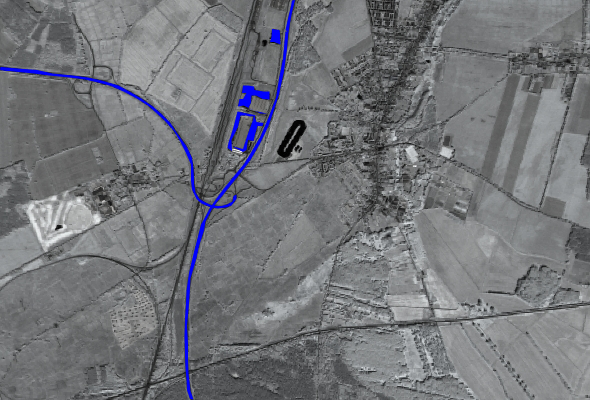
\includegraphics[scale=0.3]{src/gt_hymap02ds02_infra_highroads.jpg}}
\subfigure[ Classified roads for distance metric SAD, $k=100$, $min\_size=10$ and $min\_size2=30$]{\label{fig:nn_road_op}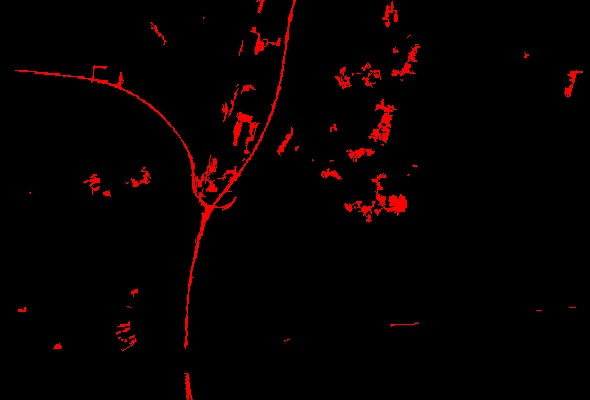
\includegraphics[scale=0.3]{src/road_op_hymap02_ds02_SAD_100_10_PP2_30.jpg}}
\caption{Nearest neighbor classifier output for test scene $1$}
\end{figure}
\forceindent Figure \ref{fig:nn_road_op} shows the classified road segments for scene$1$ using the nearest neighbor classification for distance metric SAD and parameters $k=100$, $min\_size=10$ and $min\_size2=30$. Figure \ref{fig:gt} shows the ground truth road marked in blue. The ground truth was marked manually, as the shapefile provided with the Berlin urban gradient dataset contains only few roads - specifically the small roads in urban regions. The highroads are not marked in the given shapefile. A part of the ground truth image, derived from the shapefile can be found in Figure \ref{fig:gt_shpfile}. Due to the low resolution of HyMap02 dataset, the small roads could not be marked manually and only the highroads are considered for classification. This process of manually marking the ground truth is not very accurate at pixel level.\\
\begin{wrapfigure}{l}{0.2\textwidth}
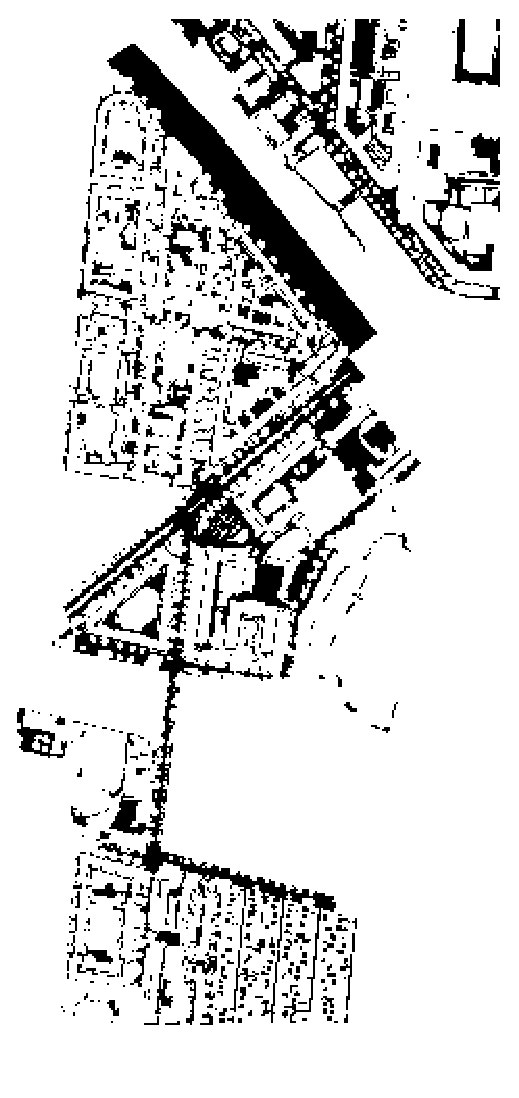
\includegraphics[width=0.2\textwidth]{src/gt_Berlin_Urban_Gradient_2009_pavement.eps}
\caption{Ground truth from Berlin-Urban-Gradient dataset showing only the small roads in urban area}
\label{fig:gt_shpfile}
\end{wrapfigure}
\forceindent Absence of proper ground truth data affects the recall, precision value of the model. The recall precision graphs for nearest neighbor classification of scene$1$ for different parameter settings are shown in Figure \ref{fig:rec_prec_sad}. The precision value varies in the range of $0.13$ to $0.21$, whereas the recall is in the range of roughly $0.5$ to $0.77$. The poor performance in terms  of numbers is because the model detects both small roads and highroads as it looks for concrete and asphalt in the input image. However, for calculating recall-precision, only the highroads are considered as correct output. The overlapping recall-precision graphs for the parameter $min\_size$ in Figure \ref{fig:rec_prec_sad} also reveals that the parameter has no effect on the performance of the model and hence, it is set arbitrarily to $10$. 
\begin{figure}[hbtp]
\centering
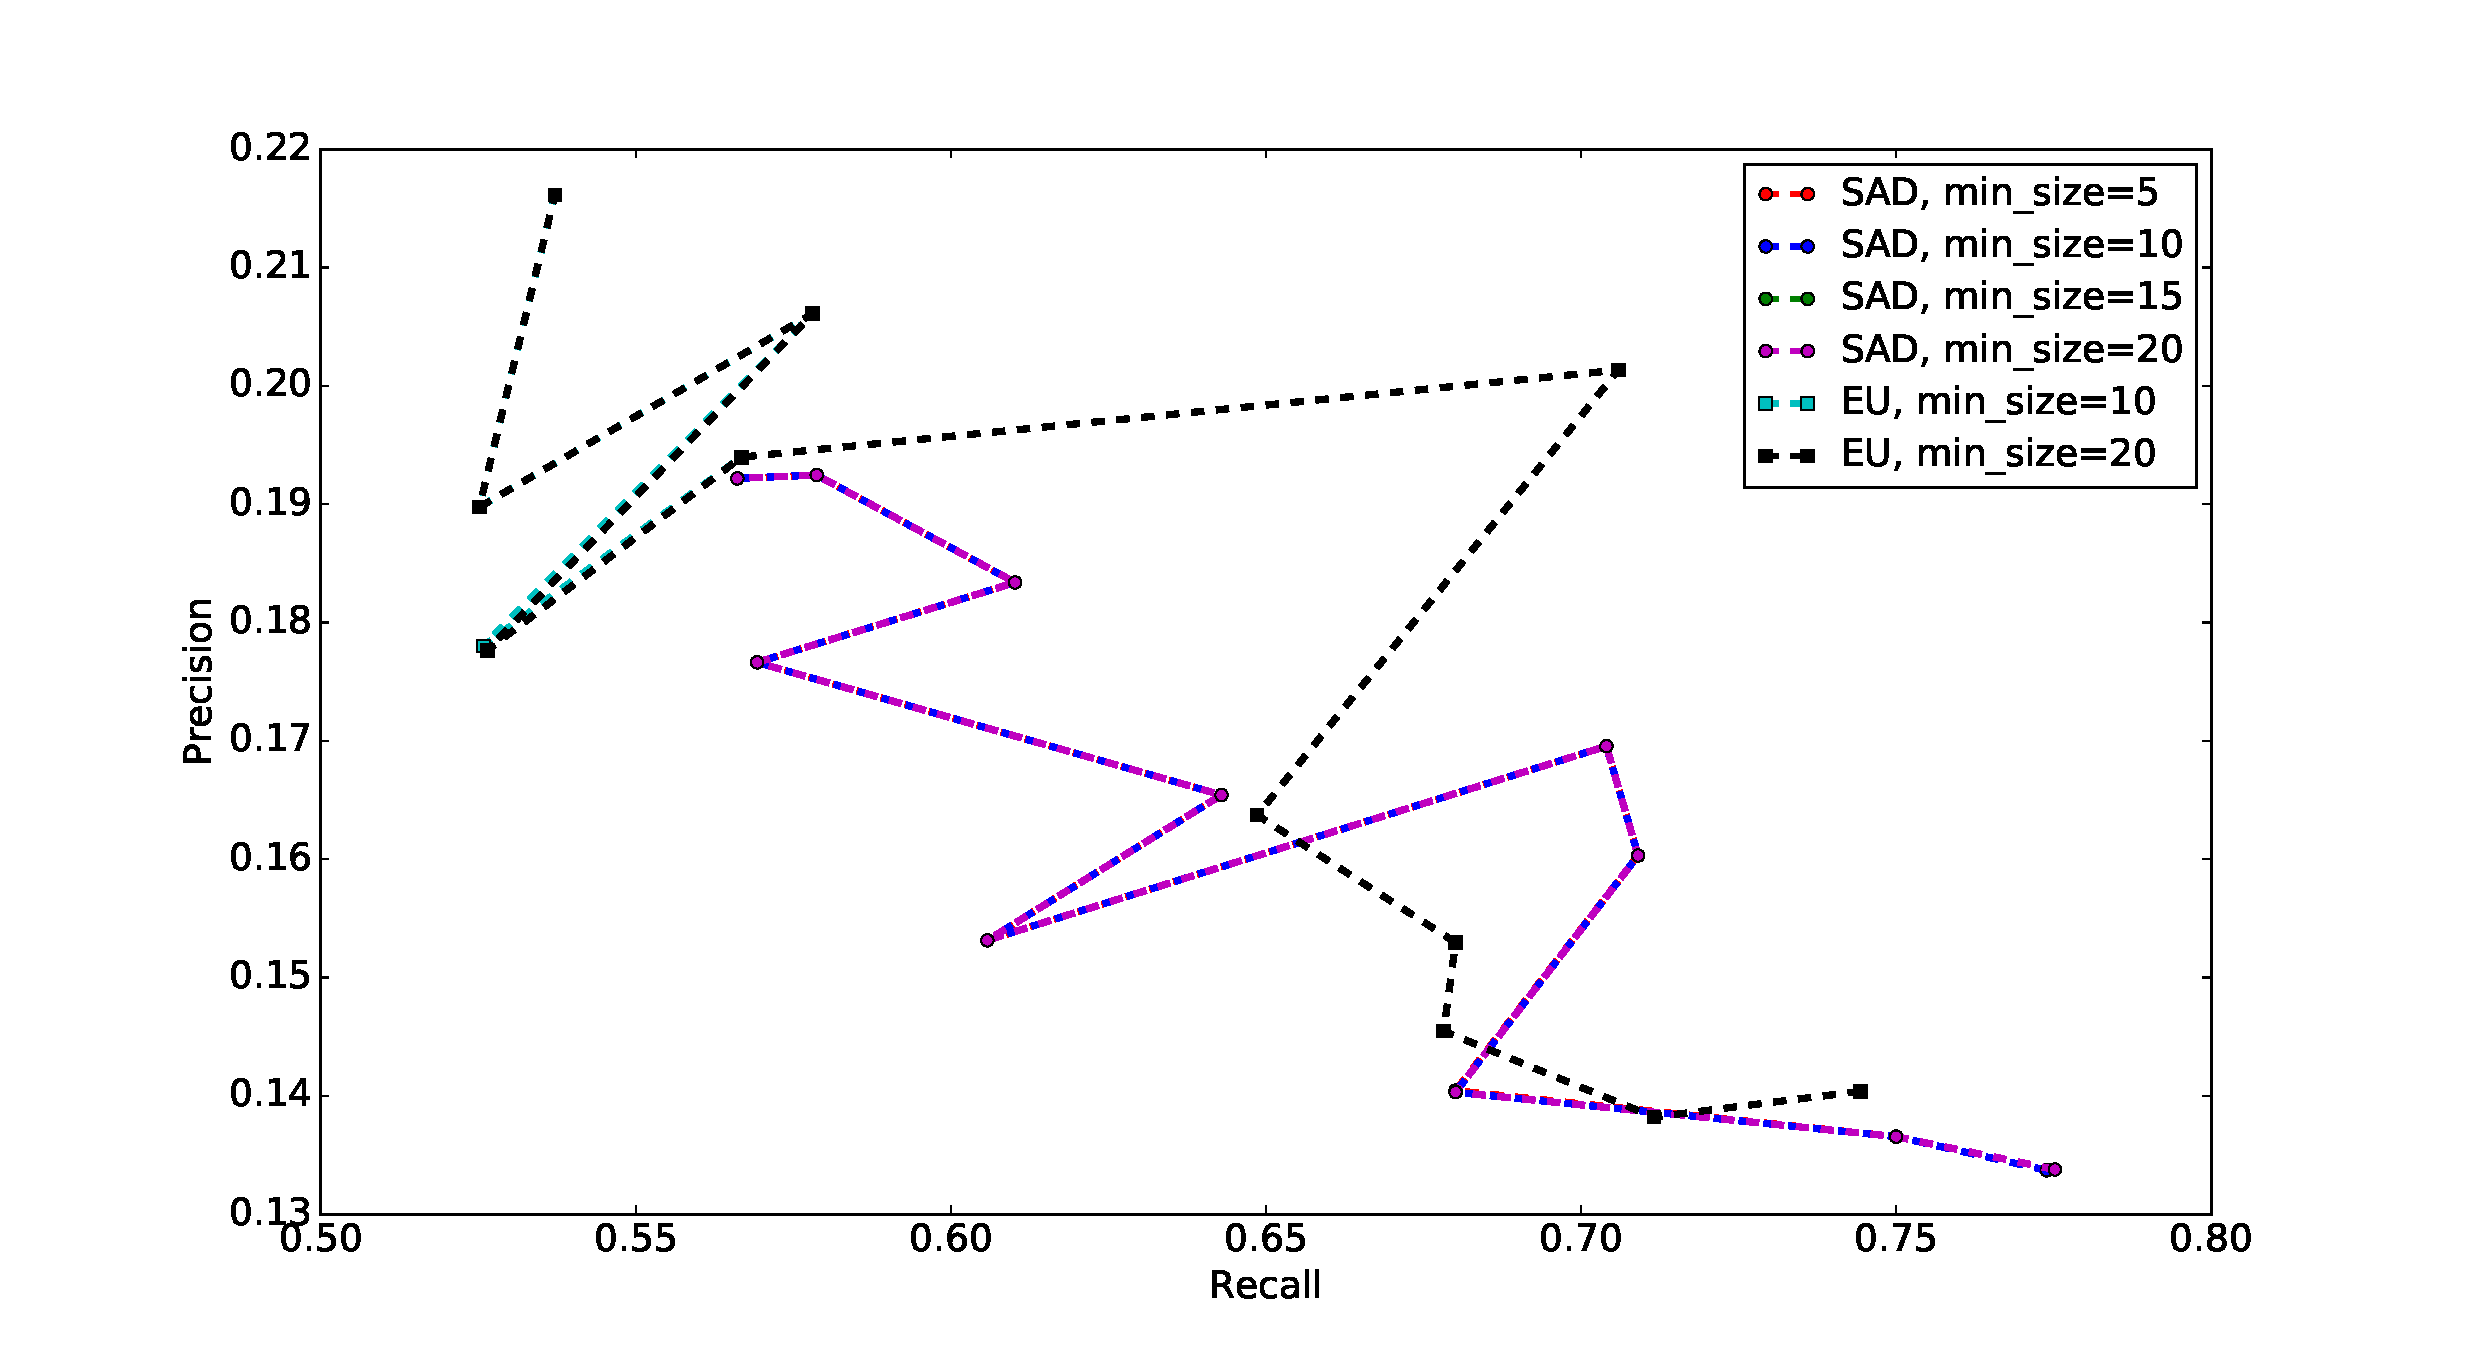
\includegraphics[width=0.9\textwidth]{src/recall_prec_graph.eps}
\caption{Recall precision graph for nearest neighbor classification of scene$1$ for distance metric SAD and EU, $k=[40,20,..140]$ and $min\_size=[5,10,15,20]$ }
\label{fig:rec_prec_sad}
\end{figure}
There is also very insignificant difference between the two distance metrics' performance. As the distance metric SAD is computationally faster, it is chosen for the final model. The parameter $k$ is set to $100$ by analysing both the recall-precision graph and the visual output.\\
\forceindent The spectral unmixing classification is also performed on scene$1$. However, the result is not promising. The recall and precision for parameters $k=100$, $min\_size=10$ and $min\_size2=30$ are $0.04$ and $0.13$ respectively. The low recall value indicates high false negatives ($1520$ occurrences). After further investigation, it is found, $99.34\%$ of the false negative pixels are mapped to category \textit{tree}. To be more specific, $77.23\%$ of these misclassified pixels are mapped to the 57th spectra, that of the \textit{deciduous tree 10}, in the spectral library.
\begin{figure}[hbtp]
\centering
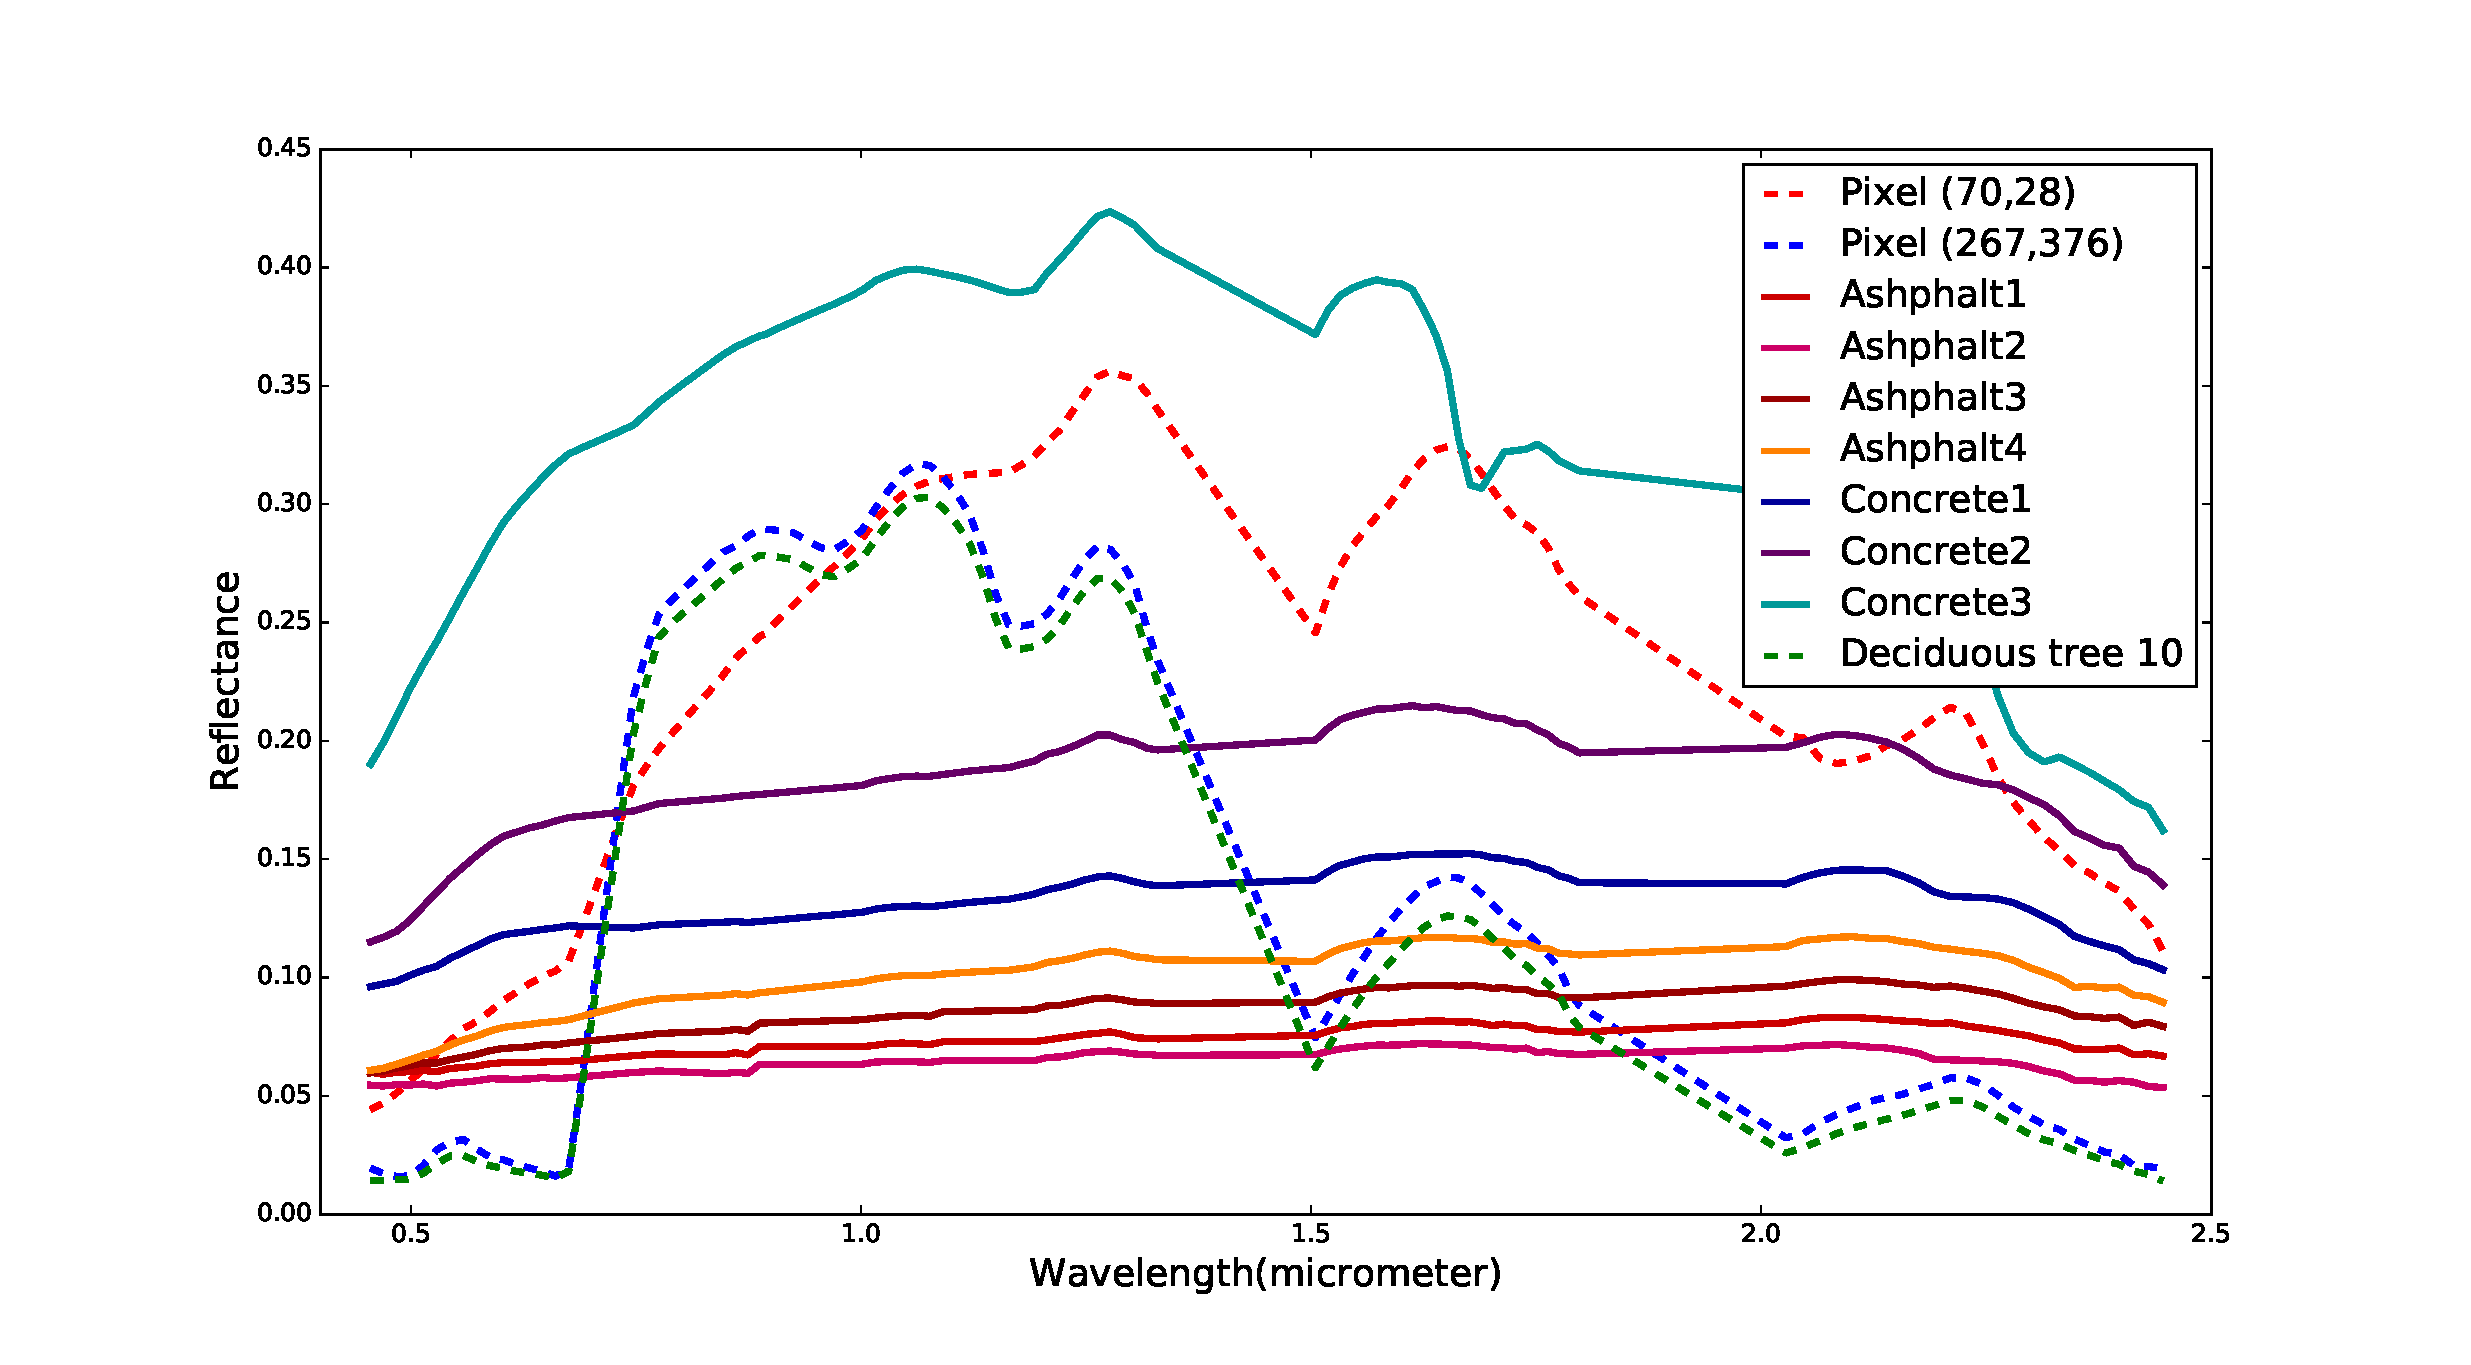
\includegraphics[width=0.9\textwidth]{src/unmix_misclassification_spectra.eps}
\caption{Spectral unmixing result analysis}
\label{fig:unmix_sp1}
\end{figure}

Figure \ref{fig:unmix_sp1} shows spectrum of such a misclassified pixel, located at $(70, 28)$ in scene$1$. The figure also plots the spectra of the different asphalt and concrete materials that constitute roads, and the \textit{deciduous tree $10$} spectrum from the spectral library. In addition to this, spectrum of a pixel, located at $(267, 376)$ in scene$1$, that is correctly classified as \textit{deciduous tree 10} is also plotted in figure \ref{fig:unmix_sp1}. It can be seen that, pixel $(70, 28)$ has similarity to the spectra of \textit{concrete} and \textit{deciduous tree $10$}. This is confirmed from the corresponding abundance vector. The highest abundance fraction for this pixel is $2.22$, which belongs to the $57^{th}$ spectra and the second highest score is $1.03$, which corresponds to the $27^{th}$ spectra, i.e. \textit{concrete$1$}. Roads are often surrounded by trees on both sides and the distribution of tree and road is quite random as opposed to the initial assumption of checker-board distribution or the linear model. This is certainly a reason behind the poor performance of the linear classifier. Moreover, the characteristic equations of the classifier, equation \ref{eq:un_abundance} and \ref{eq:fa_abundance}, do not enforce the noise factor and the non-negativity constraint of the LMM. A more sophisticated non-linear classifier would have been ideal for this kind of distribution.\\
\forceindent Based on the performance of the classifiers, the model is settled on the nearest neighbor classifier. The result of the nearest neighbor classification on the semi-urban test scene, scene$2$ with the same parameter settings as in scene$1$, can be referred to in Figure \ref{fig:nn_test}. The recall, precision value for this scene is 0.63 and 0.03 respectively. The increase in the unlabelled city roads for this scene accounts for the low precision score.

\begin{figure}[htbp]
\centering     %%% not \center
\subfigure[Scene$2$, a semi-urban sub-section from HyMap02 scene in infrared (bands R=1.0014$\mu m$, G=1.0166 $\mu m$, B=1.0318$\mu m$), with ground truth highroads marked in blue]{\label{fig:test_gt}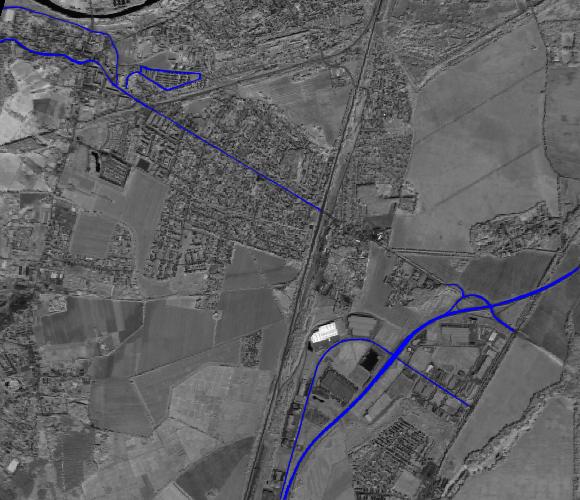
\includegraphics[scale=0.27]{src/hymap02_ds01_infra_GT_highroads.jpg}}
\subfigure[ Classified roads for distance metric SAD, $k=100$, $min\_size=10$ and $min\_size2=30$]{\label{fig:nn_test_op}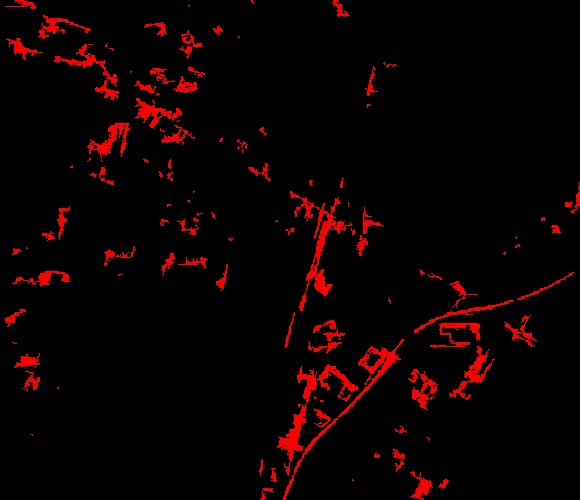
\includegraphics[scale=0.27]{src/road_op_hymap02_ds01_SAD_100_20_PP2_30.jpg}}
\caption{Nearest neighbor classifier output for test scene $2$}
\label{fig:nn_test}
\end{figure}

\section{Conclusion}
\label{sec:concl}
In this paper, a superpixel based unsupervised approach, for road detection using hyperspectral images is proposed. The model utilizes the unique characteristic spectra of road materials and the geometric properties of roads to detect road segments. It uses Felzenszwalb's segmentation algorithm to generate superpixels. Though the algorithm performs well in terms of the purpose of segmentation, it is dependent on a couple of parameters, which are set empirically. An alternative segmentation algorithm such as SLIC (simple linear iterative clustering) which relies on only one  parameter would be worth exploring as a future extension of this model. Also, the model can be extended into a fully functional road network extraction system by introducing a more advanced non-linear spectral unmixing classifier, detecting partially occluded segments, connecting road segments and extracting road centerlines.

%%%%%%%%%%%%%%%%%%%%%%%%%%%%%%%%%%%%%%
% hier werden - zum Ende des Textes - die bibliographischen Referenzen
% eingebunden
%
% Insbesondere stehen die eigentlichen Informationen in der Datei
% ``bib.bib''
%
\bibliographystyle{plain}
\bibliography{bib}

\end{document}


